\documentclass{article}
\usepackage{amsmath} % need to be on top for eps files
\usepackage{caption}
\usepackage{subcaption}
\usepackage{graphicx}
\graphicspath{ {latex/Images/} }
\usepackage{epstopdf} 


%% sidebyside images


%%%%%%%%%%%%%%%%%%%%%%%%%%%%%%%%%%%%%%%%%%%%%%%%%% Create listings (Matlab)
% % Create a matlab listing
\usepackage{listings}
\usepackage{color} %red, green, blue, yellow, cyan, magenta, black, white
\definecolor{mygreen}{RGB}{28,172,0} % color values Red, Green, Blue
\definecolor{mylilas}{RGB}{170,55,241}

\usepackage[utf8]{inputenc}
\usepackage{geometry}
 \geometry{
 a4paper,
 total={175mm,265mm},
 left=15mm,
 top=15mm,
 }
\usepackage{amsmath}%To be able to use split in equation


%%%% Include eps files:
\usepackage{amsmath} % need to be on top for eps files
\usepackage{graphicx}
%set the relative location for eps files
\graphicspath{ {/images/} }
\usepackage{listings}
\usepackage{cleveref} %cleverref needs to stand below amsmath package.
\usepackage{graphicx}
\usepackage{float}
%\usepackage{hyperref}
\usepackage{url} %To be able to use url in references
\usepackage{graphicx}
\usepackage{tabularx} % in the preamble
\usepackage{wrapfig}

%\usepackage{algorithm}
%\usepackage{algorithmic}


% To get side by side pictures:{
\usepackage{caption}
\usepackage{subcaption}
\usepackage{graphicx}




%%%%%%%%%%%%%%%%%%%%%%%%%%%%%%%%%%%%%%%%%%%%%%%%%% Create listings (Python)
% set code color pattern (for python)
% Default fixed font does not support bold face
\DeclareFixedFont{\ttb}{T1}{txtt}{bx}{n}{12} % for bold
\DeclareFixedFont{\ttm}{T1}{txtt}{m}{n}{12}  % for normal

% Custom colors
\usepackage{color}
\definecolor{deepblue}{rgb}{0,0,0.5}
\definecolor{deepred}{rgb}{0.6,0,0}
\definecolor{deepgreen}{rgb}{0,0.5,0}

\usepackage{listings}

% Python style for highlighting
\newcommand\pythonstyle{\lstset{
language=Python,
breaklines=true, % wrap lines
postbreak=\mbox{\textcolor{red}{$\hookrightarrow$}\space}, % wrap lines
basicstyle=\ttm,
otherkeywords={self},             % Add keywords here
keywordstyle=\ttb\color{deepblue},
emph={MyClass,__init__},          % Custom highlighting
emphstyle=\ttb\color{deepred},    % Custom highlighting style
stringstyle=\color{deepgreen},
frame=tb,                         % Any extra options here
showstringspaces=false            % 
}}

% Python environment
\lstnewenvironment{python}[1][]
{
\pythonstyle
\lstset{#1}
}
{}

% Python for external files
\newcommand\pythonexternal[2][]{{
\pythonstyle
\lstinputlisting[#1]{#2}}}

% Python for inline
\newcommand\pythoninline[1]{{\pythonstyle\lstinline!#1!}}


% Include path to images
\graphicspath{{images/}{latex/project1/}}

% Include pdf files in report
\usepackage{pdfpages}


\usepackage{cleveref} %cleverref needs to stand below amsmath package.
\usepackage{appendix}
\crefname{appsec}{Appendix}{Appendices} % refer to appendix as appendix iso as section (use with text in
\title{Example to plot directly into latex}
%\author{Authors:\\a-t-0}


\date{19-10-2019}
\begin{document}
\crefname{lstlisting}{listing}{listings}
\Crefname{lstlisting}{Listing}{Listings}
%%%%%%%%%%Configure matlab listing%%%%%%%%%%%%%%%%%%
% Specify matlab listing style
\lstset{language=Matlab,%
    %basicstyle=\color{red},
    breaklines=true,%
    morekeywords={matlab2tikz},
    keywordstyle=\color{blue},%
    morekeywords=[2]{1}, keywordstyle=[2]{\color{black}},
    identifierstyle=\color{black},%
    stringstyle=\color{mylilas},
    commentstyle=\color{mygreen},%
    showstringspaces=false,%without this there will be a symbol in the places where there is a space
    numbers=left,%
    numberstyle={\tiny \color{black}},% size of the numbers
    numbersep=9pt, % this defines how far the numbers are from the text
    emph=[1]{for,end,break},emphstyle=[1]\color{red}, %some words to emphasise
    %emph=[2]{word1,word2}, emphstyle=[2]{style},    
}


\maketitle
%\setcounter{chapter}{-1}
%\section{Introduction}\label{sec:intro}
Welcome, this document presents our market analysis for the TruCol consultancy. The objective of this document is to provide some basic insight into the order of magnitude of the potential of the TruCol consultancy to generate returns for its potential investors. Based on various pitch templates, \cite{kamps2020}, and private communications, we intend to convey this information through sharing our model and estimate of the following market parameters for the TruCol consultancy:

\begin{itemize}
	\item \textbf{Total addressable market (TAM)}, or total available market, is the total market demand for a product or service, calculated in annual revenue or unit sales if 100\% of the available market is achieved\cite{tam_sam_som}.
	\item \textbf{Serviceable available market (SAM)} is the portion of TAM targeted and served by a company's products or services\cite{tam_sam_som}.
	\item \textbf{Serviceable obtainable market (SOM)}, or share of market, is the percentage of SAM which is realistically reached\cite{tam_sam_som}.
\end{itemize}


\noindent Since we currently have little experience on this topic within our team, we are making our data and assumptions as transparent as possible, both in this document as in our code. This way we hope to improve our model based on your feedback by enabling you to experiment with it yourself. Additionally, because the market analysis consists of a rough estimate, three different estimation methods are used for generating the TAM, SAM and SOM estimates. The redundancy is introduced to establish some frame of reference within the results. % TODO: Improve formulation, referrence frame within the results seems counterintuitive.

The assumptions and data points for the respective models are specified in \cref{sec:assumptions}. Next, the models are described in \cref{sec:model_description} (the Python models themselves are included as appendices in \cref{app:0} to \cref{app:2} respectively). The results of these models are presented in \cref{sec:results}. To shed some light on how sensitive the model is to for example changes in assumptions, a sensitivity analysis is presented for each model in \cref{sec:sensitivity_analysis}. Next the results and sensitivity of the models are discussed in \cref{sec:discussion} and a conclusion is provided in \cref{sec:conclusion}.

We invite you to tinker with the assumptions and models yourself! The data and plots in this report are automatically updated if you run \verb+python -m code.project1.src+. If you experience any difficulties in running the code, simply reach out to us, (click on issues on the github page) and we are happy to get you running the code.
 %\newpage
%\section{Assumptions}\label{sec:assumptions}
\subsection{Top Down}\label{subsec:assumptions_top_down}

\subsection{Bottom Up}\label{subsec:assumptions_bottom_up}
\subsection{Value Theory}\label{subsec:assumptions_value_theory}
To illustrate how the python code exports the figures directly into the report, this second "hw2" is included. Below are the pictures that are created by the code listed in \cref{app:1} and \cref{app:2}.
\begin{figure}[H]
    \centering
    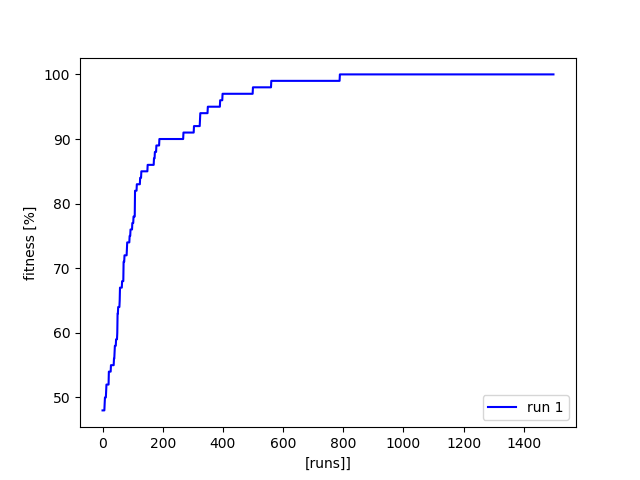
\includegraphics[width=1\textwidth]{Images/4a.png}
    \caption{Performance of some genetic algorithm}
\end{figure}

\begin{figure}[H]
    \centering
    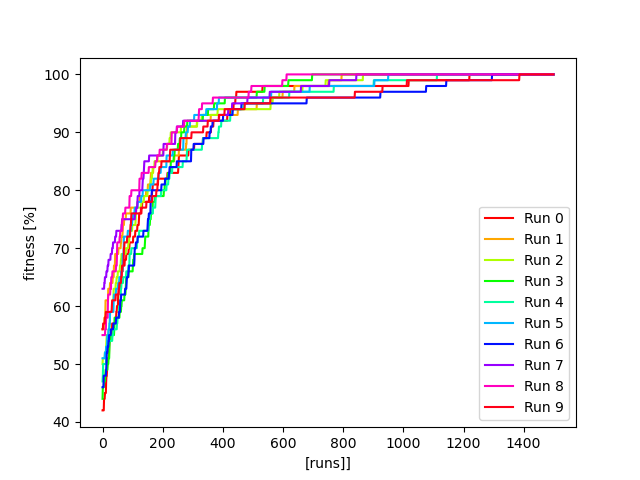
\includegraphics[width=1\textwidth]{Images/4b.png}
    \caption{Performance of some genetic algorithm}
\end{figure} %\newpage
%\input{Chapters/Conclusion.tex} %\newpage
\section{Introduction}\label{sec:intro}
Welcome, this document presents our market analysis for the TruCol consultancy. The objective of this document is to provide some basic insight into the order of magnitude of the potential of the TruCol consultancy to generate returns for its potential investors. Based on various pitch templates, \cite{kamps2020}, and private communications, we intend to convey this information through sharing our model and estimate of the following market parameters for the TruCol consultancy:

\begin{itemize}
	\item \textbf{Total addressable market (TAM)}, or total available market, is the total market demand for a product or service, calculated in annual revenue or unit sales if 100\% of the available market is achieved\cite{tam_sam_som}.
	\item \textbf{Serviceable available market (SAM)} is the portion of TAM targeted and served by a company's products or services\cite{tam_sam_som}.
	\item \textbf{Serviceable obtainable market (SOM)}, or share of market, is the percentage of SAM which is realistically reached\cite{tam_sam_som}.
\end{itemize}


\noindent Since we currently have little experience on this topic within our team, we are making our data and assumptions as transparent as possible, both in this document as in our code. This way we hope to improve our model based on your feedback by enabling you to experiment with it yourself. Additionally, because the market analysis consists of a rough estimate, three different estimation methods are used for generating the TAM, SAM and SOM estimates. The redundancy is introduced to establish some frame of reference within the results. % TODO: Improve formulation, referrence frame within the results seems counterintuitive.

The assumptions and data points for the respective models are specified in \cref{sec:assumptions}. Next, the models are described in \cref{sec:model_description} (the Python models themselves are included as appendices in \cref{app:0} to \cref{app:2} respectively). The results of these models are presented in \cref{sec:results}. To shed some light on how sensitive the model is to for example changes in assumptions, a sensitivity analysis is presented for each model in \cref{sec:sensitivity_analysis}. Next the results and sensitivity of the models are discussed in \cref{sec:discussion} and a conclusion is provided in \cref{sec:conclusion}.

We invite you to tinker with the assumptions and models yourself! The data and plots in this report are automatically updated if you run \verb+python -m code.project1.src+. If you experience any difficulties in running the code, simply reach out to us, (click on issues on the github page) and we are happy to get you running the code.
 %\newpage
\section{Assumptions}\label{sec:assumptions}
\subsection{Top Down}\label{subsec:assumptions_top_down}

\subsection{Bottom Up}\label{subsec:assumptions_bottom_up}
\subsection{Value Theory}\label{subsec:assumptions_value_theory}
To illustrate how the python code exports the figures directly into the report, this second "hw2" is included. Below are the pictures that are created by the code listed in \cref{app:1} and \cref{app:2}.
\begin{figure}[H]
    \centering
    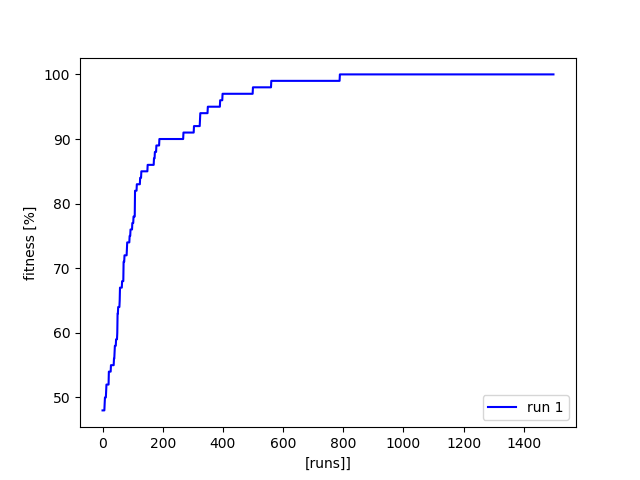
\includegraphics[width=1\textwidth]{Images/4a.png}
    \caption{Performance of some genetic algorithm}
\end{figure}

\begin{figure}[H]
    \centering
    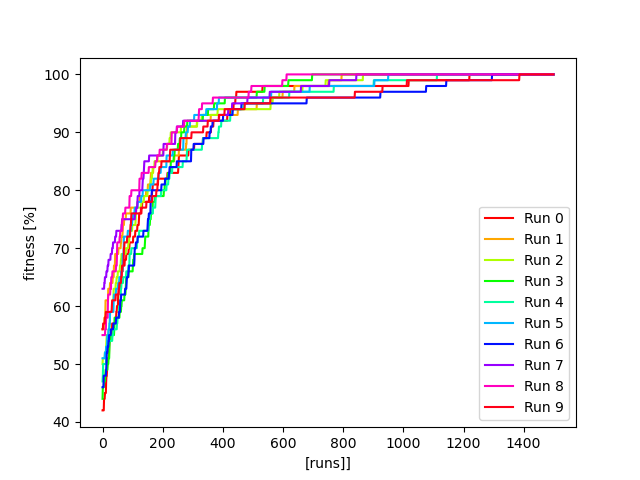
\includegraphics[width=1\textwidth]{Images/4b.png}
    \caption{Performance of some genetic algorithm}
\end{figure} %\newpage
\section{Model Description}\label{sec:model_descriptions}
\subsection{Top Down}\label{subsec:model_descriptions_top_down}
\subsection{Bottom Up}\label{subsec:model_descriptions_bottom_up}
\subsection{Value Theory}\label{subsec:model_descriptions_value_theory} %\newpage
\section{Market Analysis Model}\label{sec:market_analysis_model}
This section describes the model that is used to perform the market analysis for the TruCol company service. The model will be used to estimate the yearly revenue that is projected for this company. Typical estimation models to do this for startups are:
\begin{itemize}
	\item \textit{Top Down Model} - Starts with a large population with known size that make up the target market, and then narrows the market size down to the specific market segment.
	\item \textit{Bottom Up Model} - Takes current pricing and/or usage of product as a starting point and extrapolates up/outwards to compute the potential market size.
	\item \textit{Value Theory Model} - estimates the value provided to customers and estimates how much of that value can be reflected in the product pricing.
\end{itemize}

\noindent Since the TruCol company does not yet have a large body of current pricing and product usage, the Bottom Up Model is not used in this market analysis document. Similarly, the Value Theory Model is omitted in this market analysis as it is most powerful on historical data which is not yet available for the TruCol protocol. Since the market sizes of most sectors in which the TruCol company intends to operate, the Top Down Model is used to derive a rough estimate of the projected yearly revenue for the TruCol company.

\subsection{Top Down Model}\label{subsec:results_top_down} %\newpage
\section{Results}\label{sec:results}
\subsection{Top Down Model}\label{subsec:results_top_down}
%\subsection{Bottom Up Model}\label{subsec:results_bottom_up}
%\subsection{Value Theory Model}\label{subsec:results_value_theory}
The code listed in the appendices generated the following estimates for the total addressable market sizes for the TruCol company.
\begin{figure}[H]
    \centering
    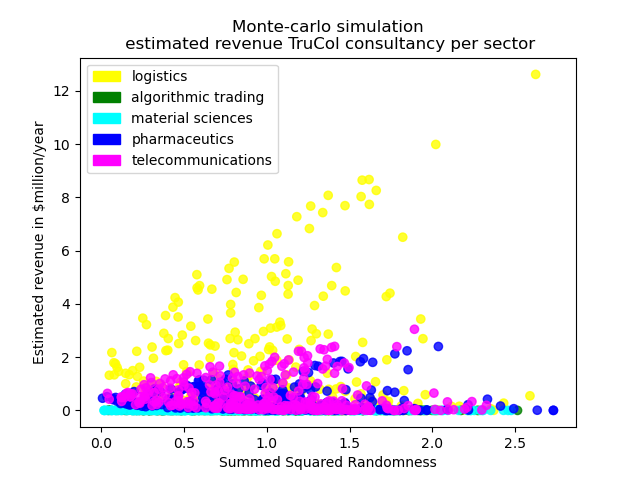
\includegraphics[width=0.5\linewidth]{Images/revenue_per_sector.png}
    \caption{A scatterplot generated by a Monte-Carlo simulation to provide an impression on the estimated projected total addressable market per sector for the TruCol company.}
    \label{fig:per_sector}
\end{figure}

\begin{figure}[H]
    \centering
    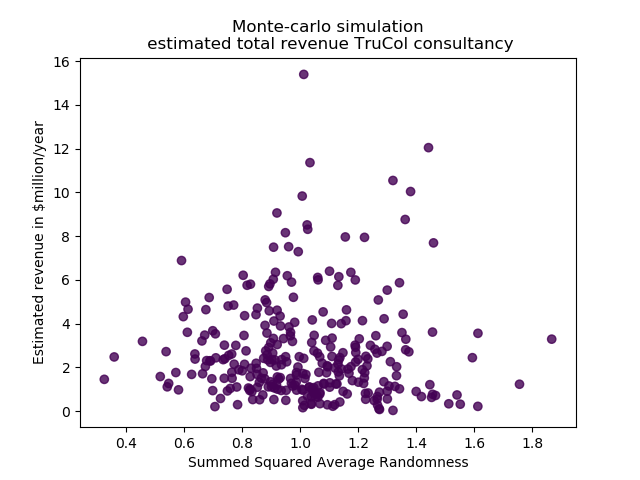
\includegraphics[width=0.5\linewidth]{Images/revenue_sum.png}
    \caption{A scatterplot generated by a Monte-Carlo simulation to provide an estimate on the projected total addressable market for the TruCol company.}
    \label{fig:summed}
\end{figure}
 %\newpage
\section{Sensitivity Analysis}\label{sec:sensitivity_analysis}
\subsection{Top Down}\label{subsec:sensitivity_analysis_top_down}
%\subsection{Bottom Up}\label{subsec:sensitivity_analysis_bottom_up}
%\subsection{Value Theory}\label{subsec:sensitivity_analysis_value_theory}
Omitted due to time constraints. Can be generated upon request. %\newpage
\section{Conclusion}\label{sec:conclusion}
A rough estimate based on various datasources has been generated to estimate the yearly revenue of the TruCol company. Additional iterations with improved datapoints is recommended to obtain a more accurate estimate. The market analysis does not yet include the growth that may be captured in diversification, emerging markets such as neuromorphic computing and in-house automation/AI-engines. Before taking these potentials into account, however, a more accurate assessment of the starting market is recommended. %\newpage










\bibliographystyle{plain} %plain style
\bibliography{references}
\addcontentsline{toc}{chapter}{Bibliography}

\begin{appendices}
\section{Appendix \_\_main\_\_.py}\label{app:a}
\IfFileExists{latex/project1/../../code/project1/src/__main__.py}{
\pythonexternal{latex/project1/../../code/project1/src/__main__.py}
}{
\pythonexternal{../../code/project1/src/__main__.py}
}
 \newpage
\section{Appendix Main.py}\label{app:2}
\pythonexternal{latex/project1/../../code/project1/src/Main.py} \newpage
\section{Appendix Model\_top\_down.py}\label{app:2}
\pythonexternal{latex/project1/../../code/project1/src/Model_top_down.py}
 \newpage
\section{Appendix Export\_code\_to\_latex.py}\label{app:0}
\pythonexternal{latex/project1/../../code/project1/src/Export_code_to_latex.py}
 \newpage
\section{Appendix Model\_value\_theory.py}\label{app:1}
\pythonexternal{latex/project1/../../code/project1/src/Model_value_theory.py}
 \newpage
\end{appendices}

\end{document}
